
\section{Introduction}
\label{sec:review:introduction}

Smurfle, gibber and other random words joined together
to make harmonious sense, as shown in Figure~\ref{fig:review:calib}
Smurfle, gibber and other random words joined together
to make harmonious sense, as shown in Figure~\ref{fig:review:calib}
Smurfle, gibber and other random words joined together
to make harmonious sense, as shown in Figure~\ref{fig:review:calib}
Smurfle, gibber and other random words joined together
to make harmonious sense, as shown in Figure~\ref{fig:review:calib}
Smurfle, gibber and other random words joined together
to make harmonious sense, as shown in Figure~\ref{fig:review:calib}
Smurfle, gibber and other random words joined together
to make harmonious sense, as shown in Figure~\ref{fig:review:calib}
Smurfle, gibber and other random words joined together
to make harmonious sense, as shown in Figure~\ref{fig:review:calib}

\begin{figure*}[thbp]
\centerline{
\begin{tabular}{cc}
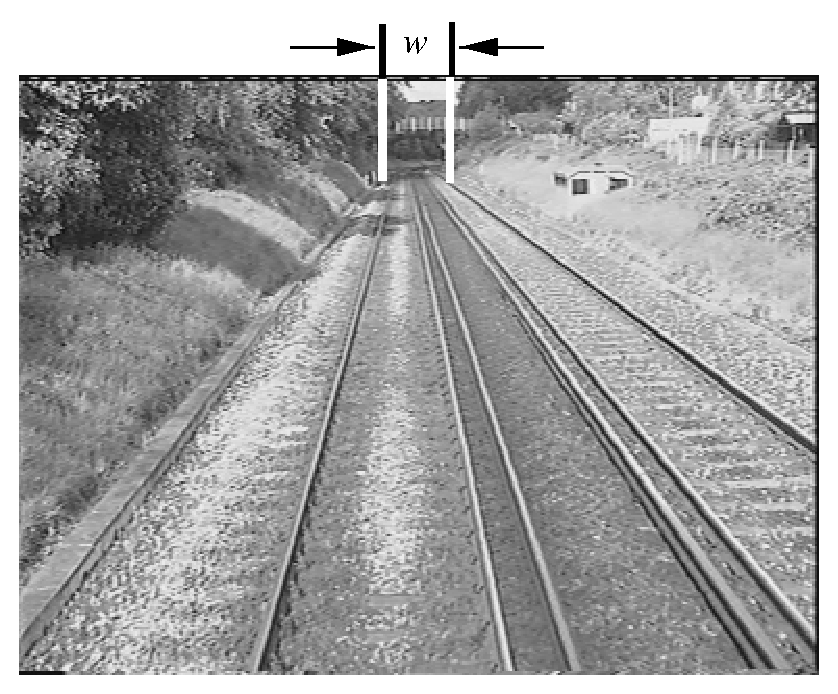
\includegraphics[width=65mm]{\localpath/Figs/calibim} &
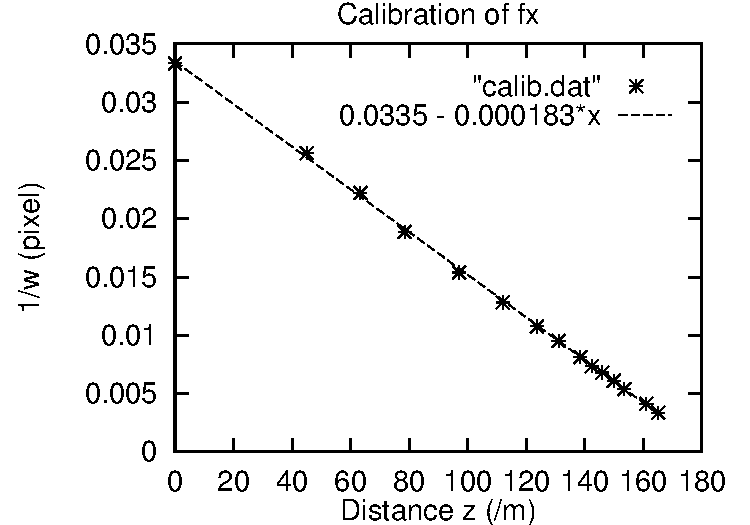
\includegraphics[width=85mm]{\localpath/Figs/calib} \\
(a) & (b)
\end{tabular}
}
\caption{\label{fig:review:calib}
(a) Image and 
(b) measured value of $1/w$ against $z$, and the fitted
straight line.
The slope 
is $1/f_xW = 1.83 \times 10^{-4}$pix$^{-1}$.m$^{-1}$
and the $z$-intercept is $D_o=183$m.
}
\hrule
\end{figure*}


Interspersed with
the smurfle, gibber and the random words joined together
to make harmonious sense, are equations like
\begin{equation}
\label{eq:review:rubbish}
a = \int_{0}^{1} x^{47} dx ~,
\end{equation}
which embody cosmic energy.




\section{Algorithms in boxes}

The concensus is that it is best to put algorithms in boxes in
figures, as illustrated in Figure~\ref{fig:review:alg1}.

\begin{figure}
\centerline{\fbox{
\begin{minipage}{75mm}
\begin{algorithmic}
\REQUIRE $n \geq 0$
\ENSURE $y = x^n$
\STATE $y \Leftarrow 1$
\STATE $X \Leftarrow x$
\STATE $N \Leftarrow n$
\WHILE{$N \neq 0$}
\IF{$N$ is even}
\STATE $X \Leftarrow X \times X$
\STATE $N \Leftarrow N / 2$
\ELSE[$N$ is odd]
\STATE $y \Leftarrow y \times X$
\STATE $N \Leftarrow N - 1$
\ENDIF
\ENDWHILE
\end{algorithmic}
\end{minipage}
}}
\caption{\label{fig:review:alg1}
An algorithm in a box for finding the value of a number taken to a
non-negative power.}
\hrule
\end{figure}

